\parindent=0em
\chapter{Rendimiento}
\pagenumbering{arabic}

\section{Teoría previa}
A la hora de evaluar un sistema podemos utilizar las siguientes métricas:
\begin{itemize}
    \item \textbf{Rendimiento}: es la cantidad de trabajo realizado por un sistema informático. Puede medirse en función de los siguientes factores.
    \begin{itemize}
        \item Tiempo de respuesta.
        \item Productividad.
        \item Utilización.
    \end{itemize}
    \item \textbf{Fiabilidad}: estabilidad y consistencia.
    \begin{itemize}
        \item Probabilidad de fallo.
        \item Tasa de fallos o tiempo medio entre fallos.
        \item Tiempo medio de reparación.
        \item Disponibilidad.
    \end{itemize}
    \item \textbf{Coste}
    \begin{itemize}
        \item Dinero.
        \item Energía.
    \end{itemize}
\end{itemize}
\subsection{Mejora de las prestaciones}
Un sistema tarda un tiempo $T_{original}$ en ejecutar un programa. Mejoramos el sistema acelerando k veces uno de sus componentes,
que se utiliza durante una fracción f del tiempo $T_{original}$
\begin{figure}[H]
    \centering
    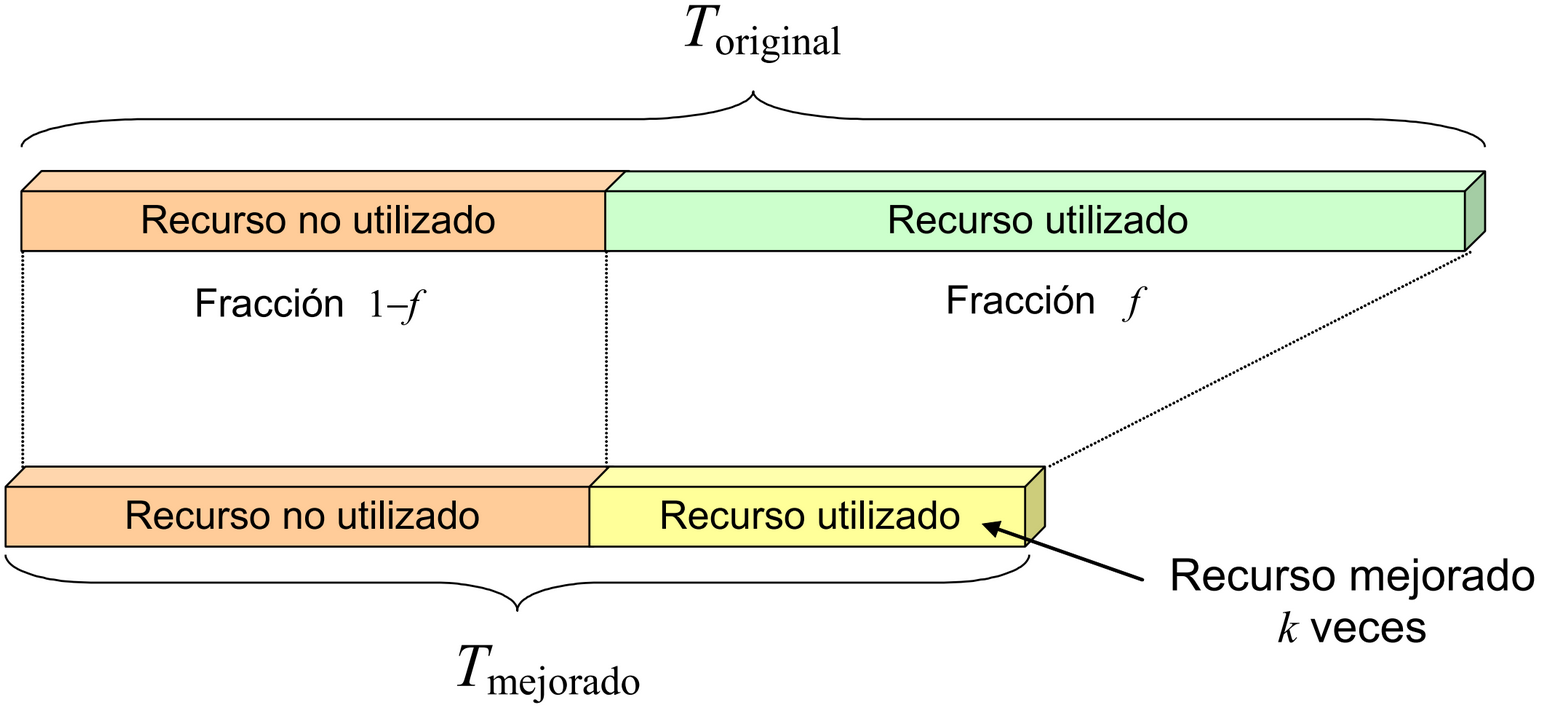
\includegraphics[width=0.9\textwidth]{Images/Mejora.png}
    \caption{Estación de servicio}
\end{figure}
\subsubsection{Ley de Amdahl}
La ley de Amdahl permite calcular la aceleración $A$ (speedup) del sistema completo después de acelerar k veces un componente que se usa una fracción f del tiempo.
\[
A=\dfrac{1}{(1-f)+(\dfrac{f}{k})}
\]

\newpage
\section{Ejercicios resueltos}
\subsection{Ejercicio 1}
\noindent
Dos computadores A y B ejecutan un programa P en 35 y 87 segundos respectivamente. El coste del computador A es de 710 euros y el del computador B de 650. ¿Cuál de ellos representa una mejor relación entre prestaciones y coste?
\begin{tcolorbox}[colback=white,colframe=cyan!50!black,fonttitle=\bfseries]


Tiempo:\\
$A\fd 35s$\\
$B\fd 87 s$\\
Coste:\\
$A\fd 710 \textup{\euro}$\\
$B\fd 650 \textup{\euro}$\\
Primero comparamos el tiempo:
\[
k=\dfrac{\text{max}}{\text{min}}=\dfrac{87}{35}=2.49=1+\dfrac{149}{100}
\]
A es un 149\% más rápido que B. Ahora comparamos el coste:
\[
\dfrac{\text{max}}{\text{min}}=\dfrac{710}{650}=1.09=1+\dfrac{9}{100}
\]
A es un 9\% más caro.
\[
\dfrac{\text{rendimiento}}{\text{coste}}\left\lbrace\begin{array}{ll}
A: \dfrac{1/35}{710}=4.024\cdot 10^{-5}\\
B: \dfrac{1/87}{650}=1.768\cdot 10^{-5}
\end{array}\right.
\]
Por tanto A representa una mejor relación rendimiento coste.
\end{tcolorbox}
\subsection{Ejercicio 2}
\noindent
Un procesador se utiliza el 83\% del tiempo en funcionamiento de un sistema informático. Si se sustituye por uno nuevo 2.5 veces más rápido ¿Cuál será el rendimiento conseguido?\\
\textbf{Nota}: Dar dicho rendimiento como aceleración global del SI.
\begin{tcolorbox}[colback=white,colframe=cyan!50!black,fonttitle=\bfseries]
f=0.83\\
k=2.5
\[
A=\dfrac{1}{1-f+\left(\dfrac{f}{k}\right)}=\dfrac{1}{0.17+\dfrac{0.83}{2.5}}=1.99=1+\dfrac{99}{100}
\]
Se consigue una mejora del 99\%.
\end{tcolorbox}
\subsection{Ejercicio 3}
\noindent
Se desea mejorar el rendimiento de un computador mediante la compra de una unidad de coma flotante, lo que permitirá reducir a la mitad el cálculo de operaciones aritméticas. Habitualmente se ejecuta una aplicación que dedica el 60\% del tiempo a la realización de cálculo aritmético. Sin unidad de coma flotante se tarda en ejecutar el programa principal 12 segundos. ¿Cuánto tiempo tardará con la nueva unidad de coma flotante?
\begin{tcolorbox}[colback=white,colframe=cyan!50!black,fonttitle=\bfseries]
f=0.6\\
k=2\\
$T_0=$12s
\[
A=\dfrac{1}{1-f+\left(\dfrac{f}{k}\right)}=\dfrac{1}{0.4+\left(\dfrac{0.6}{2}\right)}=1.43=1+\dfrac{43}{100}
\]
Mejora del 43\%.
\[
A=\dfrac{T_{\text{original}}}{T_{\text{mejorado}}}\fd T_m=\dfrac{T_0}{A}=\dfrac{12}{1.43}=8.4s
\]
\end{tcolorbox}
\subsection{Ejercicio 4}
\noindent
Con el objetivo de mejorar el rendimiento de un computador se dispone de dos opciones diferentes:
\begin{enumerate}
    \item Ampliar la memoria principal, con un coste de 250 euros consiguiendo que el 50\% de los programas (todos ellos semejantes en tiempo de ejecución) se ejecuten tres veces más rápido.
\begin{tcolorbox}[colback=white,colframe=cyan!50!black,fonttitle=\bfseries]
\textbf{Opción 1}:\\
250 \textup{\euro}\\
f=0.5\\
k=3
\[
A_1=\dfrac{1}{0.5+\dfrac{0.5}{3}}=1.5\fd 50\%\quad\text{de mejora}
\]
\end{tcolorbox}    
    \item Cambiar la placa base, con un coste de 150 euros, y con lo que el 70\% de los programas (todos ellos semejantes en tiempo de ejecución) se ejecutarán en la mitad de tiempo.
\begin{tcolorbox}[colback=white,colframe=cyan!50!black,fonttitle=\bfseries]
\textbf{Opción 2}:\\
150 \textup{\euro}\\
f=0.7\\
k=2
\[
A_2=\dfrac{1}{0.3+\dfrac{0.7}{2}}=1.54\fd 54\%\quad\text{de mejora}
\]
\end{tcolorbox}    
\end{enumerate}
¿Cuál es la mejor opción en cuanto a prestaciones y coste?
\begin{tcolorbox}[colback=white,colframe=cyan!50!black,fonttitle=\bfseries]
La opción 2 es mejor: tiene un mayor rendimiento y un menor coste (es más barata).
\end{tcolorbox} 
\subsection{Ejercicio 5}
Un programa tarda en ejecutarse un total de 124 segundos. Durante este tiempo el procesador está ejecutando tres tipos diferentes de instrucciones: aritméticas de enteros, salto y coma flotante. La proporción del tiempo de ejecución en que se emplea cada tipo es del 28, 40 y 32\% respectivamente. Se pide:
\begin{enumerate}
    \item Calcular el incremento de prestaciones si se mejoran un 15 y un 45\% las instrucciones de aritmética entera y de salto respectivamente.
\begin{tcolorbox}[colback=white,colframe=cyan!50!black,fonttitle=\bfseries]
\begin{multicols}{2}
$f_1=0.28$\\
$k_1=1.15$\\
$f_2=0.4$\\
$k_2=1.45$
\end{multicols}
Usamos la formula de Amdahl generalizada:
\[
A=\dfrac{1}{(1-\sum f)+\sum\left(\dfrac{f}{k}\right)}=\dfrac{1}{0.2+\dfrac{0.28}{1.15}+\dfrac{0.4}{1.45}}=1.19\fd\text{mejora}\quad19\%
\]
\end{tcolorbox}    
    \item Determinar cuánto se tienen que mejorar las operaciones de coma flotante si queremos rebajar el tiempo de ejecución original hasta los 95 segundos solo con esta mejora.
\begin{tcolorbox}[colback=white,colframe=cyan!50!black,fonttitle=\bfseries]
$T_m=$95s\\
$f_3=0.32$
\[
A=\dfrac{124s}{95s}=1.31s
\]
\[
A=\dfrac{1}{1-f_3+\left(\dfrac{f_3}{k_3}\right)}\fd k_3=3.72\fd\text{mejora}\quad 272\%
\]
\end{tcolorbox}    
\end{enumerate}
\subsection{Ejercicio 6}
\noindent
Un computador sin memoria caché ejecuta un programa en 180 segundos. Si se incorpora una memoria de este tipo que funcionan 15 veces más rápidamente que la memoria principal, calcúlese el porcentaje de accesos a memoria que deben satisfacerse por la memoria caché para que el programa consiga ejecutarse en 80 segundos.
\begin{tcolorbox}[colback=white,colframe=cyan!50!black,fonttitle=\bfseries]
k=15\\
$T_m=80$s\\
Nos están pidiendo calcular la $f$ de la ley de Amdahl, así que despejando nos queda:
\[
f=\dfrac{k(A-1)}{A(k-1)}=0.60
\]
\end{tcolorbox}
\subsection{Ejercicio 7}
\noindent
Una aplicación tarda en ejecutarse en una máquina secuencial 120 segundos. El administrador del sistema ha comprobado que el 70\% de las tareas de la aplicación podrían ser paralelizadas para su ejecución en un sistema multiprocesador en la nube. Se pide:
\begin{enumerate}
    \item ¿Qué aceleración experimentará la ejecución de la aplicación si el administrador contrata un sistema de 16 procesadores idénticos para la parte paralelizable? ¿En cuánto tiempo se ejecutará la aplicación? ¿Cuál será la aceleración si contrata 20, 50, 100 procesadores?
\begin{tcolorbox}[colback=white,colframe=cyan!50!black,fonttitle=\bfseries]
f=0.7\\
k=16\\
$t_A=$120s
\[
A=\dfrac{1}{1-f+\dfrac{f}{k}}=\dfrac{1}{(1_k-0.7)+\dfrac{0.7}{16}}=2.91
\]
Calculamos de la misma manera los resultados para las otras 3 situaciones, y nos queda:
\[\left\lbrace\begin{array}{lll}
k=20\fd A=2.98\\
k=50\fd A=2.4\\
k=100\fd A=3.25
\end{array}\right.
\]
\end{tcolorbox}    
    \item ¿A qué tiempo de ejecución podría reducirse el cómputo sin reprogramar la aplicación?
\begin{tcolorbox}[colback=white,colframe=cyan!50!black,fonttitle=\bfseries]
Calculamos el límite de A suponiendo infinitos procesadores:
\[
\lim_{k\to\infty}A = 3.3
\]
Y sacamos el tiempo mejor:
\[ % Ya casi tengo los grafos pepine
t_{\text{mej}}=\dfrac{t_0}{A}=\dfrac{120}{3.3}=36s
\]
\end{tcolorbox}    
\end{enumerate}
\subsection{Ejercicio 8}
\noindent
Durante la fase de diseño de un computador se ha introducido una mejora que incrementa en un factor k=10 el rendimiento local de un cierto recurso. Esta mejora ha permitido reducir el tiempo de ejecución original de un programa. Una vez introducida la mejora se ha podido estimar que ésta se emplea durante el 50\% del tiempo mejorado.
\begin{enumerate}
    \item ¿Cuál es el porcentaje del tiempo original de ejecución del programa afectado por la mejora?
\begin{tcolorbox}[colback=white,colframe=cyan!50!black,fonttitle=\bfseries]
\begin{figure}[H]
    \centering
    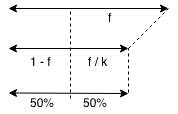
\includegraphics[width=0.3\textwidth]{Images/18.png}
\end{figure}
Podemos igualar las dos mitades y sacamos el valor de $f$:
\[
1-f=\dfrac{f}{k}\fd 10-10f-f=0\fd f=0.9090
\]
\end{tcolorbox}    
    \item ¿Cuál es la aceleración global conseguida?
\begin{tcolorbox}[colback=white,colframe=cyan!50!black,fonttitle=\bfseries]
\[
A=\dfrac{1}{1-0.909+\left(\dfrac{0.909}{10}\right)}=5.5
\]
\end{tcolorbox}    
\end{enumerate}
\subsection{Ejercicio 9}
\noindent
Consideremos un computador dedicado exclusivamente a la gestión de reserva de billetes en un aeropuerto regional donde el procesador actual, que funciona a 66 MHz, es el cuello de botella, con una utilización media del 84\% (el 16\% restante se usa en tareas de entrada/salida). Se pide determinar cuál de las dos opciones siguientes para reemplazar el procesador presenta la mejor relación entre prestaciones y coste.\\

En ambos casos se supone que el computador admite los dos procesadores y que no hace falta recompilar la aplicación de reserva de billetes.
\begin{enumerate}
    \item Procesador Bart a 550 MHz, con un precio de 480 euros.
\begin{tcolorbox}[colback=white,colframe=cyan!50!black,fonttitle=\bfseries]
\textbf{Opción a}:
\[
k_1=\dfrac{\text{max}}{\text{min}}=\dfrac{550}{66}=8.3
\]
\[
C_1=480\textup{ \euro}
\]
\[
A_1=\dfrac{1}{0.16+\dfrac{0.84}{8.3}}=3.83
\]
\[
\dfrac{A_1}{C_1}=0.0079
\]
\end{tcolorbox}    
    \item Procesador Homer a 500 MHz, con un precio de 270 euros.
\begin{tcolorbox}[colback=white,colframe=cyan!50!black,fonttitle=\bfseries]
\textbf{Opción b}:
\[
k_2=\dfrac{500}{60}=7.57
\]
\[
C_2=270\text{euros}
\]
\[
A_2=\dfrac{1}{0.16+\dfrac{0.84}{7.57}}=3.69
\]
\[
\dfrac{A_2}{C_2}=0.013
\]
\end{tcolorbox}    
\end{enumerate}
\begin{tcolorbox}[colback=white,colframe=cyan!50!black,fonttitle=\bfseries]
Puesto que $\dfrac{A_2}{C_2}>\dfrac{A_1}{C_1}$, el procesador Homer es mejor.

\end{tcolorbox}
\subsection{Ejercicio 10}
\noindent
Un computador ejecuta una aplicación de gestión de base de datos. Cada transacción con esta base de datos tarda un total de 12 segundos. Un análisis llevado a cabo mediante un monitor de ejecución de programas ha permitido averiguar que el 78\% del tiempo que tarda cada transacción se debe al acceso del subsistema de discos, mientras que el resto del tiempo se emplea en operaciones del procesador.
\begin{enumerate}
    \item Calcúlese el nuevo tiempo de respuesta de una transacción si el subsistema de discos se sustituye por uno nuevo cuatro veces más rápido.
\begin{tcolorbox}[colback=white,colframe=cyan!50!black,fonttitle=\bfseries]
\[
A=\dfrac{1}{1-f+\left(\dfrac{f}{4}\right)}=2.414
\]
\[
A=\dfrac{T_A}{T_D}\fd T_D=\dfrac{T_A}{A}=4.98s
\]
\end{tcolorbox}    
    \item Repítase el apartado anterior suponiendo que el subsistema de discos se sustituye por uno nuevo seis veces más rápido.
\begin{tcolorbox}[colback=white,colframe=cyan!50!black,fonttitle=\bfseries]
\[
A=\dfrac{1}{1-f+\left(\dfrac{f}{6}\right)}=2.85
\]
\[
T_D=\dfrac{T_A}{A}=4.21
\]
\end{tcolorbox}    
    \item Determínese la mejora del rendimiento obtenida en cada una de las actualizaciones anteriores.
\begin{tcolorbox}[colback=white,colframe=cyan!50!black,fonttitle=\bfseries]
\[
\dfrac{4.98}{4.21}=1.18
\]
\end{tcolorbox}    
\end{enumerate}
\subsection{Ejercicio 11}
\noindent
Un programa de simulación se ejecuta en 280 segundos. El 70\% del tiempo utiliza el procesador y el resto utiliza el disco.
\begin{enumerate}
    \item Determina el tiempo de ejecución con un procesador tres veces más rápido.
\begin{tcolorbox}[colback=white,colframe=cyan!50!black,fonttitle=\bfseries]
k=3\\
A=1.875
\[
T_D=\dfrac{T_A}{A}=149.33
\]
\end{tcolorbox}    
    \item Calcula la fracción del tiempo mejorado de ejecución durante el cual se utiliza el nuevo procesador. Haz un análisis del fenómeno observado.
\begin{tcolorbox}[colback=white,colframe=cyan!50!black,fonttitle=\bfseries]
\[
280\cdot 0.3=84
\]
\[
T_{\text{mej}}=149.33-84=65.33
\]
\[
x=\dfrac{65.33\cdot 100}{144.31}=43.75\%
\]
\end{tcolorbox}    
    \item A raíz del resultado obtenido en el apartado anterior, si hubiéramos de mejorar este sistema actualizado, ¿sobre qué componente del mismo deberíamos incidir?
\begin{tcolorbox}[colback=white,colframe=cyan!50!black,fonttitle=\bfseries]
Deberíamos cambiar el dispositivo que más frecuencia de uso tenga.
\end{tcolorbox}    
\end{enumerate}
\subsection{Ejercicio 12}
\noindent
Sean dos factores de mejora sobre un sistema $k_1$=5 y $k_2$=3. Suponiendo que ambas mejoras no se pueden hacer de manera simultánea, calcula la relación entre las fracciones de tiempo $f_1$ y $f_2$ durante las cuales se han de emplear las mejoras para que ambas obtengan la misma aceleración global.
\begin{tcolorbox}[colback=white,colframe=cyan!50!black,fonttitle=\bfseries]
\[
\dfrac{1}{1-f_1+\dfrac{f_1}{5}}=\dfrac{1}{1-f_2+\dfrac{f_2}{3}}
\]
\[
1-f_1+\dfrac{f_1}{5}=1-f_2+\dfrac{f_2}{3}
\]
\[
f_2=\dfrac{12}{10}f_1
\]
\end{tcolorbox}
\subsection{Ejercicio 13}
\noindent
El tiempo medio de respuesta de un sitio web es de 15 segundos. El 55\% de este tiempo es utilizado por el subsistema de discos, mientras que el resto es utilizado por el procesador. Se pretende reducir este tiempo por debajo de los 10 segundos. Indica cuál de las siguientes opciones es mejor:
\begin{enumerate}
    \item Adquirir un nuevo procesador un 50\% más rápido.
\begin{tcolorbox}[colback=white,colframe=cyan!50!black,fonttitle=\bfseries]
k=2.5\\
A=1.17
\[
T_D=\dfrac{T_A}{A}=12.75s
\]
\end{tcolorbox}    
    \item Sustituir el subsistema de discos por uno 2,5 veces más rápido que el actual.
\begin{tcolorbox}[colback=white,colframe=cyan!50!black,fonttitle=\bfseries]
$T_{\text{disco}}=8.28$\\
$T_{\text{proc}}=6.75$\\
k=2.5\\
A=1.49
\[
T_D=\dfrac{T_P}{A}=10.06s
\]
Ninguno de los dos mejora.
\end{tcolorbox}    
\end{enumerate}
\subsection{Ejercicio 14}
\noindent
Un sistema multiprocesador está configurado con un número fijo de 6 procesadores y la aceleración conseguida con un programa es igual a 3.
\begin{enumerate}
    \item ¿Cuál es la fracción paralelizable $f$ del programa?
\begin{tcolorbox}[colback=white,colframe=cyan!50!black,fonttitle=\bfseries]
Despejamos $f$ de la formula de Amdahl:
\[
3=\dfrac{1}{1-f+\left(\dfrac{f}{6}\right)}\fd f=0.8\fd 80\%
\]
\end{tcolorbox}    
    \item Si la versión secuencial del programa se ejecuta en 325 segundos, ¿en cuánto tiempo lo hará con la actual configuración del multiprocesador?
\begin{tcolorbox}[colback=white,colframe=cyan!50!black,fonttitle=\bfseries]
\[
T_A=325\fd T_0=\dfrac{T_A}{A}=\dfrac{325}{3}=108.3s
\]
\end{tcolorbox}    
    \item ¿Podría reducirse el tiempo de ejecución por debajo de 55 segundos ampliando el número de procesadores hasta 32?
\begin{tcolorbox}[colback=white,colframe=cyan!50!black,fonttitle=\bfseries]
\[
t_{\text{mej}}=T_A\cdot\left(0.2+\dfrac{0.8}{32}\right)=73.13s
\]
No se consigue.
\end{tcolorbox}    
    \item ¿Y con 16 procesadores y reduciendo a la mitad la fracción no paralelizable?
\begin{tcolorbox}[colback=white,colframe=cyan!50!black,fonttitle=\bfseries]
La fracción no paralelizable es $1-f = 0.2$, por tanto si la reducimos a la mitad su valor será $0.1$, y por tanto $f=0.9$.
\[
t_{\text{mej}}=325\cdot\left(0.1+\dfrac{0.9}{16}\right)=50.78s
\]
Sí, se consigue.
\end{tcolorbox}    
\end{enumerate}